\begin{frame}
\frametitle{The tip-labeled time-tree}

A tip-labeled time-tree is described by a {\it tip-labeled ranked topology} of size $k$ and {\it coalescent intervals}, $\mathbf{u} = \{u_2, \dots, u_k\}$.

\medskip{}

\begin{centering}

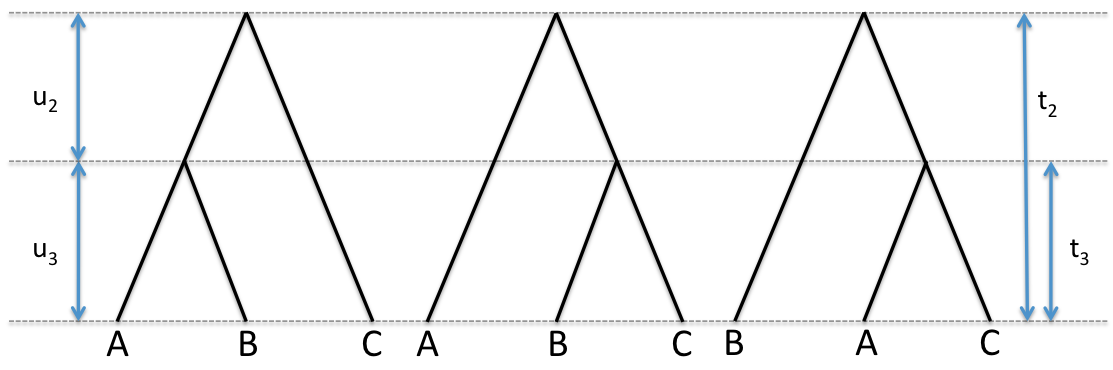
\includegraphics[width=\textwidth]{../images/timetree3}

\end{centering}

\medskip{}

These time-trees of size 3 can be interpreted as describing the possible alternative evolutionary histories or (uniparental) ancestries of the three individuals represented by the labeled tips.


\end{frame}
